%% main.tex -- COLLIE, IEEE UV 2026 submission draft.
%%
%% Venue: 8th IEEE International Conference on Universal Village (IEEE UV 2026).
%% Format: IEEEtran conference class, two column, US Letter.
%% Page budget and every other venue fact, with the URL it was verified at and
%% the access date, are recorded in manuscript/README.md. Where a fact could not
%% be verified, README.md names the assumption used instead.
%%
%% THIS IS AN INITIAL DRAFT. Experiments are still running. Every result cell,
%% every arm score, and every contrast is marked with \pending{...} and is listed
%% in the placeholder inventory in manuscript/README.md. Every substantive claim
%% is traced to its evidence in manuscript/CLAIMS.md.

\documentclass[conference]{IEEEtran}
\IEEEoverridecommandlockouts

%%% --- required by IEEEtran ----------------------------------------------------
\usepackage{cite}

%%% --- encoding ----------------------------------------------------------------
\usepackage[T1]{fontenc}
\usepackage[utf8]{inputenc}

%%% --- math --------------------------------------------------------------------
\usepackage{amsmath,amssymb,amsfonts}
\usepackage{bm}
%% IEEEtran already defines \proof / \endproof, so amsthm must be told to take
%% them over rather than error on a redefinition.
\let\proof\relax
\let\endproof\relax
\usepackage{amsthm}
\newtheorem{theorem}{Theorem}
\newtheorem{lemma}{Lemma}

%%% --- graphics and color ------------------------------------------------------
\usepackage{graphicx}
\graphicspath{{figures/}}
\usepackage{xcolor}
\usepackage{tikz}
\usetikzlibrary{arrows.meta,positioning,fit,calc,backgrounds,decorations.pathreplacing}
\usepackage{pgfplots}
\pgfplotsset{compat=1.18}

%%% --- tables ------------------------------------------------------------------
\usepackage{booktabs}
\usepackage{array}
\usepackage{multirow}

%%% --- captions ----------------------------------------------------------------
\usepackage{caption}
\captionsetup[table]{font={footnotesize,sc},labelsep=period}
\captionsetup[figure]{font={footnotesize},name={Fig.},labelsep=period}

%%% --- microtype and refs -----------------------------------------------------
\usepackage{url}
\usepackage[hidelinks]{hyperref}

%%% --- the placeholder convention ---------------------------------------------
%% Every number, figure datapoint, and result sentence that the experiments have
%% not yet produced is wrapped in \pending. The convention is mandatory: a
%% half-filled draft must be impossible to mistake for a finished one. Grep
%% "pending" over manuscript/ and the count must match the inventory table in
%% manuscript/README.md exactly.
%%
%% \pending is a TEXT command. It must never appear inside a math environment.
\newcommand{\pending}[1]{\textcolor{red}{\textbf{[PENDING: #1]}}}
%% Table cells that will receive a single scalar. Same convention, shorter.
\newcommand{\pcell}{\textcolor{red}{\textbf{PENDING}}}

%%% --- notation shorthands ----------------------------------------------------
\newcommand{\Filt}{\mathcal{F}}
\newcommand{\Ind}{\mathbb{1}}
\newcommand{\Real}{\mathbb{R}}
\newcommand{\Prob}{\mathbb{P}}
\newcommand{\Expect}{\mathbb{E}}
\newcommand{\shockspec}{\textsc{ShockSpec}}
\newcommand{\controlconfig}{\textsc{ControlConfig}}
\newcommand{\alertspec}{\textsc{AlertSpec}}
\newcommand{\eprocess}{e\nobreakdash-process}
\newcommand{\evalue}{e\nobreakdash-value}
\newcommand{\collie}{\textsc{Collie}}
\newcommand{\evalpath}{\texttt{eval/}}
\newcommand{\envpath}{\texttt{env.py}}

\begin{document}

%% No manual line breaks: IEEEtran centres and wraps a title better than a
%% hand-chosen break, which rewrapped badly at this length.
\title{Ask What Changed, Not What to Order: Typed Shock Hypotheses,
Compiled into an Inventory Controller, Activated by an Anytime-Valid
\eprocess{}}

%% AUTHOR LINE, non-anonymous. Review is NOT blind: the IEEE UV 2026 call for
%% papers (verified 2026-09-17, URL and quote in manuscript/README.md) contains
%% no mention of blind or anonymous review, the venue's own annotated sample
%% ships a full \author block with affiliations and emails, and the submission
%% instructions distribute no anonymous style file. The names themselves are
%% \pending{} because the author list is the submitting authors' to set.
%%
%% The call also asks submissions to carry no running headers or footers, no page
%% numbering, and no blue underlining on URLs and email addresses. IEEEtran's
%% conference mode already omits headers and page numbers, this file adds no
%% fancyhdr block, and hyperref is loaded with [hidelinks] for the third.
\author{\IEEEauthorblockN{\pending{author list}}
\IEEEauthorblockA{\pending{affiliation}\\
\pending{email}}}

\maketitle

\begin{abstract}
A language model can be attached to a deployed replenishment controller in three
separable ways: by changing \emph{when} it is consulted, \emph{what} it may say,
and \emph{when} its answer is trusted. Published agentic inventory systems change
all three at once, so no reported gain can be attributed to any of them. We
separate the three. \collie{} consults a frozen language model only at rare
trigger moments, and the model may return only a typed hypothesis about the
exogenous process, a \shockspec{}, drawn from a closed vocabulary of six shock
families and frozen at the proposal period. A deterministic compiler maps that
hypothesis onto one point of a 72 configuration grid for a capped base-stock
controller, which computes every order, and the hypothesis influences orders only
after an anytime-valid \eprocess{} started strictly after the proposal crosses
the Ville threshold $1/\alpha_j$ under the geometric budget
$\alpha_j = \alpha\,2^{-j}$ over at most two proposals per episode. The resulting
guarantee is a model-conditional, anytime-valid, per-episode false-activation
bound, and we state explicitly what it does not cover. The testbed is an audited
reimplementation of InventoryBench whose accounting matches the official pipeline
exactly and whose operations research baseline reproduces all 1{,}320 published
order sequences bit for bit. That reproduction surfaced a harness divergence: the
published baseline score of $0.4447$ belongs to the legacy simulator, while the
same policy scores $0.5208$ under the authoritative submission path. We evaluate
an eleven-rung arm ladder with physical and charged call accounting kept
separate. \pending{headline result}
\end{abstract}


\begin{IEEEkeywords}
large language models, inventory control, operations research, anytime-valid
inference, \eprocess{}, sequential change detection, agent evaluation
\end{IEEEkeywords}

\section{Introduction}

Retailers are already asking language models what to order. On InventoryBench, a
benchmark of 1{,}320 multi-period lost-sales replenishment instances, the
strongest published language-model strategy reaches a normalized reward of
$0.5380$ against $0.4447$ for the operations research policy it is asked to
improve~\cite{inventorybench}. That gap is why the approach is taken seriously.
It is also uninterpretable: the published strategy calls the model once per
period, lets it name an order quantity outright, and applies that quantity with
no test of whether the model was right, so three decisions are welded into one
design and the reported gain cannot be assigned to any of them.

Reproducing the baseline made this worse. Our arm~1 reimplements the published
capped base-stock policy and matches all 1{,}320 published order sequences bit
for bit, so it is the same policy rather than an approximation of one. Under the
benchmark's authoritative submission path that policy scores $0.5208$, not
$0.4447$, because the published figure came from the benchmark's legacy
simulator, which keeps a lost shipment visible in in-transit inventory forever
and so makes the baseline under-order after every loss. The motivating evidence
is therefore both bundled and partly artifactual, and the useful question is not
whether a language model helps on average but which of the three decisions does
the work.

\subsection*{The thesis}

A language model should not be asked what to order. It should be asked what
changed, once, in a vocabulary the system fixed in advance, and it should be
believed only after the data says so.

\collie{} implements that in three stages. A shared trigger decides \emph{when}:
an alert or a calibrated detector opens a proposal opportunity, a refractory
window suppresses repeats, and at most two proposals are permitted per episode. A
closed schema decides \emph{what}: at the proposal period $\tau_j$ the model
returns a \shockspec{}, a typed claim about the exogenous process drawn from a
registered vocabulary of families, directions, onset windows, magnitude bins and
durations, and it cannot write an order, a threshold, a likelihood, a falsifier,
or code. An anytime-valid \eprocess{} decides \emph{whether}: the hypothesis is
frozen at $\tau_j$ and influences no order until evidence arriving strictly after
$\tau_j$ drives the process above $1/\alpha_j$, and until then a deterministic
compiler is the only thing that ever touches the baseline controller's
parameters. Our notes name the design axis in one line: compile shocks, or always
inventory. Either the model's reading of an exception is compiled once into the
controller and then defended by prospective evidence, or the model is asked what
to order, every period, forever.

%% fig1_pipeline.tex -- Figure 1. The whole idea in one picture.
%%
%% FINAL FIGURE DESCRIPTION (for the illustrator, and for the record):
%% A left-to-right pipeline across the full text width, with a side panel.
%%   Left, stacked: the two trigger inputs, an operational alert and the demand
%%   telemetry stream. They meet in the trigger box, which is annotated with the
%%   refractory window of 5 periods and the cap of at most 2 proposals.
%%   The trigger opens a proposal opportunity at the stopping time tau_j.
%%   The language model is consulted exactly there and returns one typed
%%   ShockSpec, drawn with a lock icon to mark that it is frozen and immutable.
%%   The compiler maps the spec to one of 72 registered ControlConfig points.
%%   Between the compiler and the controller sits the e-process gate, drawn as a
%%   valve rather than an arrow, because that is the point of the figure: the
%%   compiled configuration is computed but does not flow until the evidence
%%   path E_{j,t}, accumulated only from observations after tau_j, crosses
%%   1/alpha_j. A dashed bypass path carries the baseline configuration straight
%%   to the controller and is the live path while the gate is closed.
%%   The controller emits q_t. A feedback arrow returns the realized observation
%%   Y_{t+1} to both the telemetry stream and the evidence path, which is what
%%   makes the closed-loop argument of Lemma 1 necessary rather than decorative.
%%   Right panel: the eleven-rung ladder as a vertical list, with arms 8, 9 and
%%   10 braced together and labeled "one physical call set, three activation
%%   policies", and arm 10 marked as the contribution.
%%
%% This file is the real figure, drawn in TikZ with base libraries only. It is
%% included by \input, not \includegraphics, so no external build step exists.

\begin{figure*}[!t]
\centering
\footnotesize
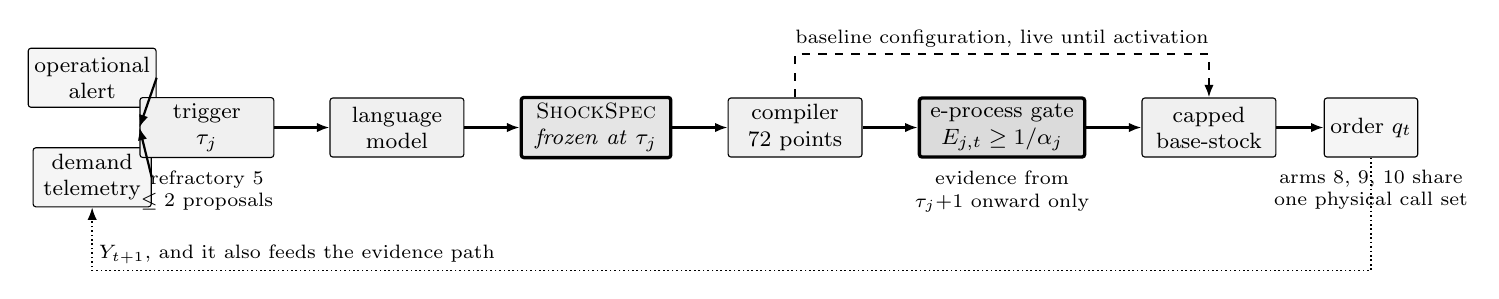
\begin{tikzpicture}[
  node distance=3.6mm,
  box/.style={draw, rounded corners=1pt, align=center, inner sep=2.2pt,
              minimum height=7.5mm, font=\footnotesize},
  src/.style={box, fill=black!4, minimum width=15mm},
  proc/.style={box, fill=black!6, minimum width=17mm},
  spec/.style={box, fill=black!10, minimum width=19mm, very thick},
  gate/.style={box, fill=black!14, minimum width=21mm, very thick},
  outbox/.style={box, fill=black!4, minimum width=11mm},
  rung/.style={align=left, font=\scriptsize, inner sep=1pt},
  flow/.style={-{Latex[length=1.6mm]}, thick},
  bypass/.style={-{Latex[length=1.6mm]}, thick, dashed},
  fb/.style={-{Latex[length=1.6mm]}, semithick, densely dotted},
  lbl/.style={font=\scriptsize, align=center, inner sep=1pt},
]

%% ---- inputs ---------------------------------------------------------------
\node[src] (alert) {operational\\alert};
\node[src, below=5mm of alert] (tele) {demand\\telemetry};

%% ---- trigger --------------------------------------------------------------
\node[proc, right=6mm of $(alert)!0.5!(tele)$] (trig) {trigger\\$\tau_j$};
\node[lbl, below=1.2mm of trig] {refractory 5\\$\le 2$ proposals};

%% ---- model ---------------------------------------------------------------
\node[proc, right=7mm of trig] (llm) {language\\model};

%% ---- the frozen spec ----------------------------------------------------
\node[spec, right=7mm of llm] (spec) {\shockspec{}\\\emph{frozen at} $\tau_j$};

%% ---- compiler ------------------------------------------------------------
\node[proc, right=7mm of spec] (comp) {compiler\\72 points};

%% ---- the gate ------------------------------------------------------------
\node[gate, right=7mm of comp] (gate)
  {\eprocess{} gate\\$E_{j,t} \ge 1/\alpha_j$};
\node[lbl, below=1.2mm of gate] {evidence from\\$\tau_j{+}1$ onward only};

%% ---- controller and order ------------------------------------------------
\node[proc, right=7mm of gate] (ctrl) {capped\\base-stock};
\node[outbox, right=6mm of ctrl] (order) {order $q_t$};

%% ---- flow ----------------------------------------------------------------
\draw[flow] (alert.east) -- (trig.west);
\draw[flow] (tele.east)  -- (trig.west);
\draw[flow] (trig)  -- (llm);
\draw[flow] (llm)   -- (spec);
\draw[flow] (spec)  -- (comp);
\draw[flow] (comp)  -- (gate);
\draw[flow] (gate)  -- (ctrl);
\draw[flow] (ctrl)  -- (order);

%% ---- the baseline bypass, live while the gate is closed ------------------
\coordinate (bypassL) at ($(comp.north) + (0,5.5mm)$);
\coordinate (bypassR) at ($(ctrl.north) + (0,5.5mm)$);
\draw[bypass] (comp.north) |- (bypassL) -- (bypassR) -| (ctrl.north);
\node[lbl, above=0.4mm] at ($(bypassL)!0.5!(bypassR)$)
  {baseline configuration, live until activation};

%% ---- closed loop ---------------------------------------------------------
\coordinate (fbY) at ($(tele.south) + (0,-8mm)$);
\draw[fb] (order.south) |- (fbY) -| (tele.south);
\node[lbl, above=0.4mm] at ($(fbY) + (26mm,0)$) {$Y_{t+1}$, and it also feeds the evidence path};

%% The ladder side panel was removed once Table~\ref{tab:ladder} carried the same
%% eleven rungs; keeping both duplicated the list and made this figure a third of
%% a page taller. The brace annotation that mattered is kept inline below.
\node[lbl, below=1.2mm of order] {arms 8, 9, 10 share\\one physical call set};

\end{tikzpicture}
\caption{The handshake. A shared trigger decides \emph{when} the model is
consulted, a closed schema decides \emph{what} it may say, and an
anytime-valid \eprocess{} decides \emph{whether} the answer touches an order.
The gate is drawn as a valve rather than an arrow because that is the point: the
compiled configuration is computed immediately and flows only after evidence
gathered strictly after $\tau_j$ drives $E_{j,t}$ above $1/\alpha_j$. The dashed
path is the baseline configuration, which is live until then. The dotted return
is what makes fact (F1) of Section~\ref{sec:verify} load-bearing rather than
decorative, since the controller's own orders shape the observations the test
consumes.}
\label{fig:pipeline}
\end{figure*}


One episode threads through the paper. A planner is told that a carrier has
suspended outbound scans on a lane and that containers booked over the last week
may not arrive at all. This is family~5 of our generator, a lost-shipment burst in
which orders dispatched in one to three consecutive periods are never delivered,
and it is a hard case on purpose: the demand stream is untouched, so the
calibrated detector fires at its null rate and the shortfall shows up in
telemetry only as an arrival that does not happen. Text is the only early signal,
and a wrong reading of it is expensive in both directions.

\subsection*{Contributions}

\begin{itemize}\itemsep0pt
\item \textbf{An audited testbed, and a divergence finding.} Our runner matches
      the official pipeline with a maximum absolute difference of exactly $0.0$
      over 648 comparisons, and arm~1 reproduces every published baseline order
      sequence bit for bit, which is how we established that the published score
      belongs to the legacy simulator (Section~\ref{sec:background}).
\item \textbf{\shockspec{} and its compiler.} A closed, frozen, typed vocabulary
      for what changed, plus a total deterministic map from a hypothesis to one
      point of a 72 configuration grid over a capped base-stock controller
      (Sections~\ref{sec:spec}, \ref{sec:compile}).
\item \textbf{Per-episode anytime-valid activation.} A discrete-mixture
      likelihood-ratio \eprocess{} started strictly after the proposal, with
      budget $\alpha_j = \alpha\,2^{-j}$ over at most two proposals, a
      family-by-family validity statement, and one explicitly prohibited shortcut
      (Section~\ref{sec:verify}).
\item \textbf{An eleven-rung ladder with honest cost accounting,} in which arms
      8, 9 and 10 share one physical set of proposal calls, so a difference
      between them cannot be a difference in calls (Section~\ref{sec:ladder}).
\end{itemize}

This draft is written against a running experiment, so every result cell is
marked \pending{} and inventoried, and Section~\ref{sec:notclaim} states the
single guarantee the system certifies and enumerates the readings of it that are
wrong.

\section{The Audited Benchmark}
\label{sec:background}

What does InventoryBench specify, and what did we have to establish ourselves? We
answer from its code and its data, because three answers differ from its
documentation and one of them moves a published number.

\textbf{Inventory and lead times.} There are 1{,}320 instances, 720 synthetic and
600 derived from real weekly apparel sales, split evenly across three lead-time
directories. Synthetic episodes run 50 decisions and real ones 47, not the 48
often reported, which counts the trajectory file's header line. Two lead-time
quantities are easy to conflate: the \emph{promised} lead time, passed to the
policy at initialization with values $\{0, 4, 2\}$, and the \emph{actual}
per-period lead time, never shown to the policy, with values $\{0\}$, $\{4\}$ or
$\{1,2,3,\infty\}$, where $\infty$ encodes a lost shipment. Exactly 440 instances,
the whole stochastic third, contain at least one lost period.

\textbf{Event order and observability.} Each period decides, then receives, then
sells, then charges. Two consequences are load-bearing: an order with actual lead
time zero arrives in the same period, because scheduling precedes the arrival
pop, and the in-transit total shown at $t$ still contains units that land at $t$.
Holding falls on ending inventory and nothing is backordered, which makes
lost-sales units a coherent safety endpoint. The policy sees uncensored previous
demand rather than sales, and in-transit inventory is a scalar with no shipment
ages, so many shipment-level histories are consistent with the same receipts.
That last fact drives a decision in Section~\ref{sec:verify}: the controller may
keep an imputed first-in-first-out ledger, and the verifier may never use it as
evidence.

\textbf{Integer economics, and two absences.} Every demand, profit and holding
cell is an integer, so every sum is exact and our equivalence suite can demand a
maximum absolute difference of exactly $0.0$ rather than a tolerance: a nonzero
difference could only be a semantic disagreement. Holding cost is $1.0$ everywhere
and profit is $19$, $4$ or $1$, so \textbf{the labels \texttt{high},
\texttt{med} and \texttt{low} name the margin, not the holding burden}. Two
absences are ours to fill. There is no upstream order cap, so \collie{} registers
its own $C_t$ and labels it as ours wherever it affects a number, distinct from
the published baseline's internal smoother. And a transit pause is not
expressible in the instance format, because both simulators fix a shipment's
arrival period at order time, so it needs a project-owned sidecar.

\subsection{The harness divergence}
\label{sec:divergence}

The benchmark ships two simulators and they disagree about one thing. In the
legacy game simulator a lost order stays in in-transit inventory forever, since
its arrival period is set to infinity and never popped, while in the submission
path it is never added to in-transit at all. The disagreement never changes the
physics, since replaying a run's orders under the other simulator reproduces the
arrivals, the reward and the lost-unit total exactly. It changes what a policy
\emph{reads}, because a base-stock policy under legacy semantics credits units
that will never arrive, orders less, and loses fewer units.

We declare the submission path authoritative, because it is the contract we are
scored against. Under legacy semantics our reimplementation reproduces the
published $0.4447$ to one unit in the last place and matches all 1{,}320 published
order sequences bit for bit, a far stronger check than a matching aggregate that
many policies could reach. Under the authoritative path the same policy scores
$0.5208$, exactly the 880 deterministic-lead-time instances still match, and all
440 stochastic ones differ. Since 440 is precisely the number of instances the
audit found to contain a lost shipment, the divergence is accounted for with no
residue. The published figure was therefore generated under legacy lost-order
semantics and is not reachable from the submission path, so every table comparing
against it must name the harness.

\section{Problem Setup}
\label{sec:setup}

What must the information structure respect for a sequential test to be
legitimate inside a closed control loop?

Let $I_t$ be on-hand inventory at the start of period $t$, $P_t$ the aggregate
in-transit total, $A_t$ our order, $R_t$ aggregate receipts, and $p$ and $h$ the
per-unit profit and holding cost. The order is coerced and capped as
$A_t = \min(\max(0, \lceil q_t \rceil), C_t)$ and dispatched with a latent
transit time, and our endpoints accumulate profit and lost sales under the audited
event order. Let $Y_t$ be the exposed observable,
uncensored demand in the headline setting, and $\Filt_t$ the sigma-algebra
generated by every observation through period $t$, taken \emph{immediately
before} $A_t$ is chosen. Two properties follow. \textbf{(A1) Actions are
predictable:} $A_t$ is $\Filt_t$-measurable, and the runner builds and freezes
the observation before calling the controller, so this holds by construction
rather than by convention. \textbf{(A2) Actions affect only the future:} $A_t$
influences $Y_{t+1}$ and later, never $Y_t$. Conditioning $Y_r$ on
$(\Filt_{r-1}, A_{r-1})$ is therefore well defined and does not condition on
anything $A_{r-1}$ could have altered retroactively, and every density below is
written that way. A zero actual lead time moves $R_t$ rather than $Y_t$, so (A2)
survives. Finally, $\tau_j$ is the proposal period of hypothesis $j$ and a
stopping time, $h_j$ the \shockspec{} frozen there, and $E_{j,t}$ its evidence
process.

\section{\shockspec{}: The Typed Commitment}
\label{sec:spec}

What is the model allowed to say? Exactly one object, drawn from a vocabulary the
system froze before any test episode ran. Closing that vocabulary is what makes
the later test admissible rather than decorative.

At the proposal period $\tau_j$ the model receives only information in
$\Filt_{\tau_j}$: the permitted product text, any alert visible then, the demand
and arrival history, the inventory position, an aged pipeline summary and the
costs. It must return valid JSON under a closed schema that
forbids unknown keys and yields an immutable object. The model selects nine
fields. \texttt{shock\_family} is one of \texttt{no\_change},
\texttt{demand\_level}, \texttt{temporary\_pulse}, \texttt{lead\_time\_shift},
\texttt{shipment\_loss}, \texttt{transit\_pause} or \texttt{compound}.
\texttt{target\_stream} ranges over demand, arrival, both and none, and
\texttt{direction} over the six registered directions. \texttt{onset\_window} is
a registered offset pair or null, while \texttt{magnitude\_bin},
\texttt{persistence} and \texttt{duration\_bin} take their registered bins.
\texttt{evidence\_refs} points at visible message spans or observation
identifiers, and \texttt{prospective\_signature} is schema-defined. Five fields
are stamped by the system and never by the model:
$\tau_j$, the one-based proposal index, the model identifier, the decoding hash
and the prompt hash. \texttt{no\_change} is a first-class output rather than a
failure code, and an accepted abstention is scored separately from a formatting
failure because capability and reliability should not share a cell.
\texttt{transit\_pause} is a first-class family even though no generator family
emits it alone, since it is the supply leg of family 6.

The model selects a key. It cannot write a falsifier, a likelihood, a threshold,
an order equation, or code: the system maps the pair (\texttt{shock\_family},
\texttt{prospective\_signature}) to a verifier construction and the whole object
to controller parameters. An invalid object gets one format-repair attempt, a
second failure falls back to the unchanged baseline, and every attempt is counted
as accepted, accepted after repair, or fallback. The restriction is load-bearing:
if the model could invent its own vague test after seeing the trigger window,
falsifiability would be cosmetic. Two structural facts remove the
circularity. \textbf{(A3) Closed selection space:} the hypothesis is drawn from a
registered vocabulary whose map to a construction is frozen. \textbf{(A4) Frozen
at a stopping time:} $\tau_j$ is a stopping time, $h_j$ is
$\Filt_{\tau_j}$-measurable, and its evidence product starts at $\tau_j + 1$. For
the carrier suspension the model is expected to return \texttt{shipment\_loss} on
the \texttt{arrival} stream, direction \texttt{arrival\_interrupted}, duration bin
\texttt{1\_3}, with \texttt{evidence\_refs} naming the alert and the arrival
residual. Nothing in that object is an order. It says what changed.

\section{Compilation: From a Claim to an Order}
\label{sec:compile}

How does a sentence about the world become an order quantity? Through a total,
pure, deterministic function with no episode state, history or clock.

A \controlconfig{} is a four-tuple $(m, L_{\mathrm{eff}}, \gamma, k)$ with
$m \in \{0.6, 0.75, 1.0, 1.25, 1.5, 2.0\}$, $L_{\mathrm{eff}} \in \{1,2,3,4\}$
and $\gamma \in \{0, 0.5, 1\}$, which is $6 \times 4 \times 3 = 72$
configurations. The fourth entry is a pure function of the other three, obtained
by comparing the point against the grid reference on two flags, whether the
compiled belief moves demand and whether and how it moves the supply side. That
key has two consumers: control acts on it, and Section~\ref{sec:verify}'s
registry resolves the same key into the construction that will test it, so a
hypothesis cannot be acted on under one reading and tested under another. Note
that $L_{\mathrm{eff}}$ is a compiled \emph{belief} and never the observation's
promised lead time, because the compiler is a pure function of the \shockspec{}
alone. Precedence is fixed as family, then direction, then magnitude bin, then
target stream.

\begin{table}[!tb]
\caption{The registered compiler table, by severity rank, as absolute points
around the grid reference $(1, 1, 1)$.}
\label{tab:mapping}
\centering
\footnotesize
\begin{tabular}{@{}llll@{}}
\toprule
Shape & $m$ & $L_{\mathrm{eff}}$ & $\gamma$ \\
\midrule
\texttt{demand\_level} up      & 1.25 / 1.5 / 2.0 & 1 & 1.0 \\
\texttt{demand\_level} down    & 0.75 / 0.6 / 0.6 & 1 & 1.0 \\
\texttt{temporary\_pulse} up   & 1.25 / 1.5 / 2.0 & 1 & 1.0 \\
\texttt{temporary\_pulse} down & 0.75 / 0.6 / 0.6 & 1 & 1.0 \\
\texttt{lead\_time\_shift}     & 1.0 & 2 / 3 / 4 & 1.0 \\
\texttt{shipment\_loss}        & 1.0 & 1 & 0.5 / 0.0 / 0.0 \\
\texttt{transit\_pause}        & 1.0 & 2 / 2 / 3 & 1.0 / 1.0 / 0.5 \\
\texttt{compound}              & 1.25 / 1.25 / 1.5 & 2 / 2 / 3 & 1.0 \\
\texttt{no\_change}            & 1.0 & reference & 1.0 \\
\bottomrule
\end{tabular}
\end{table}

A lead-time shift moves $L_{\mathrm{eff}}$ alone, because arrivals are still
coming, while a shipment loss moves $\gamma$ alone, because arrivals keep their
timing but fewer can be trusted to be real. A pause is deliberately asymmetric,
since under the authoritative harness nothing inflates the pipeline count for
$\gamma$ to correct. Composition is reference-relative, because an absolute grid
point applied wholesale would move axes the hypothesis does not concern, and a
demand-up hypothesis compiled to $L_{\mathrm{eff}} = 1$ against a promised lead
time of 2 cancels its own demand signal exactly. An axis left at the reference is
inherited, and a moved axis applies absolutely for $m$, as an offset for
$L_{\mathrm{eff}}$ and as a ratio for $\gamma$.

One controller serves every arm that routes through the compiler, differing only
in which configuration is active in a period. With $\bar{d}_t$ and $s_{d,t}$ the
running mean and sample standard deviation of the training samples followed by
every demand observed so far, and $z^\star = \Phi^{-1}(p/(p+h))$,
\begin{align}
IP_t &= I_t + \gamma P_t, \\
S_t  &= m\,(1 + L_{\mathrm{eff}})\,\bar{d}_t
        + z^\star \sqrt{1 + L_{\mathrm{eff}}}\; s_{d,t}, \\
q_t  &= \min\bigl(\max(0, \lceil S_t - IP_t \rceil),\; C_t,\; \hat{C}_t\bigr).
\end{align}
The critical fractile is read from the per-period cost columns rather than
assumed constant, putting $z^\star$ at the $0.95$, $0.80$ and $0.50$ quantiles
across the three registered cost ratios, and $\hat{C}_t$ is the published
baseline's own internal smoother, kept separate from our cap $C_t$ because they
are different objects that share a word. The property that makes the ladder
legitimate is that at the per-instance baseline configuration this controller
reproduces arm~1 bit for bit, so ``the published operations research policy is
running'' is literally true for every arm while no hypothesis is active. For the
running example the compiled point is $\gamma = 0.5$ at low severity and
$\gamma = 0$ above it, so the inventory position shrinks by the discounted
pipeline and the controller replaces the shipments it no longer believes in. That
is the whole intervention.

\section{Verified Activation}
\label{sec:verify}

When may a frozen hypothesis touch an order? Only when observations that arrived
after it was written down have paid for the privilege.

\subsection{Construction and theorem}

The model chooses $h_j$ \emph{because} something looked unusual, and reusing the
periods that motivated the choice as confirming evidence would make the apparent
evidence an artifact of selection, and (A3) and (A4) remove that. For a
proposal $j$ with registered null $p_0$ and alternative region $\Theta_j$,
\begin{equation}
E_{j,t} \;=\; \int_{\Theta_j}
\prod_{r=\tau_j+1}^{t}
\frac{p_{h_j,\theta}\bigl(Y_r \mid \Filt_{r-1}, A_{r-1}\bigr)}
     {p_0\bigl(Y_r \mid \Filt_{r-1}, A_{r-1}\bigr)}
\; dW_j(\theta),
\label{eq:eprocess}
\end{equation}
with $E_{j,\tau_j} = 1$ by the empty-product convention. Two facts
make~\eqref{eq:eprocess} an \eprocess{} started at $\tau_j$~\cite{ramdas-savi,
e-detectors}. \textbf{(F1) Unit conditional mean:} for fixed $\theta$ the ratio has conditional
expectation one under the null, because the expectation integrates it against
$p_0$ and leaves $\int p_{h,\theta}\, d\mu = 1$, which needs only a common
dominating measure and $p_0 > 0$ wherever $p_{h,\theta} > 0$, and we check that
shared support rather than assume it. \textbf{(F2) Mixing preserves the property:} the
fixed-$\theta$ product is a nonnegative martingale with unit initial value, a
test martingale, and a mixture over $\theta$ with prior $W_j$ is again one by
Fubini, which handles a composite alternative without estimating $\theta$ from
the data being tested.

(F1) is where the closed loop is handled, because it holds \emph{whatever policy
generated} $A_{r-1}$, including one that reacts to $E_{j,t}$ itself, so an
adaptive, self-referential controller does not invalidate the test. That is why
the design insists actions be predictable. One implementation detail is easy to
get wrong: with $W_j$ discrete on a registered grid, the mixture sits
\emph{outside} the product, so each component carries its own cumulative ratio
and the prior averages component wealth. Multiplying period-wise mixture averages
would define a different process.

Ville's inequality bounds a nonnegative supermartingale $M$ with $M_0 = 1$ by
$\Prob(\sup_t M_t \ge 1/\alpha) \le \alpha$~\cite{ville}. Index proposals within
episode $e$ by $j = 1, 2, \dots$, allocate $\alpha_j = \alpha\, 2^{-j}$, and
activate proposal $j$ at the first $t$ with $E_{j,t} \ge 1/\alpha_j$.

\begin{theorem}
\label{thm:activation}
Under the registered global no-change null, with (A1) through (A4) and (F1),
(F2),
$\Prob_0(\text{any false activation in episode } e)
\le \sum_j \alpha_j \le \alpha \sum_{j \ge 1} 2^{-j} = \alpha$.
\end{theorem}

Each $E_{j,\cdot}$ is a unit-initial nonnegative martingale, so Ville bounds its
own crossing probability by $\alpha_j$, and a union bound with
$\sum_{j\ge1} 2^{-j} = 1$ gives the result. The allocation is why the proposal
index is one-based: an index of zero would spend the whole budget on the first
proposal.

\subsection{Arrivals, and the one prohibited shortcut}

Only the aggregate receipt is observed, and many shipment-level histories are
consistent with the same receipt sequence, so \emph{assuming} first-in-first-out
order would inject an assumption as if it were data. The controller's imputed
ledger is a control convenience only and the verifier marginalizes instead, which
is enforced rather than documented: the ledger's symbols are unreachable from the
verifier by a static check and a runtime input-graph assertion. Our own dispatch
quantities are known exactly, so the only latent quantity is each outstanding
order's transit realization, and the state is the vector of remaining transit
times of outstanding cohorts, truncated at $L_{\max}$ with a lost outcome
absorbing, giving at most $1296$ states for $L_{\max} = 4$. A forward recursion
over that state returns the \emph{exact} conditional density of the receipt, so
(F1) applies verbatim, with exactness checked per family against brute force.

Compound shocks need one more rule, because the generator's
conditional-independence flag is false there. Where the contract makes
independence explicit a registered \emph{joint} conditional likelihood may be
used. Otherwise we run two separate \eprocess{}es with an explicit prior split of
the budget, and Theorem~\ref{thm:activation} applies with the finer partition,
because the union bound is indifferent to how the budget is subdivided in
advance. Multiplying marginal likelihood ratios when independence is not part of
the contract is \textbf{prohibited}: under dependence the product is not the
ratio of joint densities, its conditional mean need not be one, (F1) fails, and
the bound is void with no visible symptom. The joint code path is therefore
asserted unreachable whenever the flag is false, since an assertion is the only
defense that survives a refactor.

\subsection{Validity, lifecycle, and what we do not claim}
\label{sec:notclaim}

A registered validity status accompanies every family and the code is asserted to
agree with it, so a disagreement is a test failure. The two demand families use
the mixture ratio and are anytime-valid, with the pulse underpowered by
construction. The three arrival families and the compound family use the forward
recursion, with a budget split for the compound case, and are anytime-valid
\emph{on our own episodes only}, since the official lead-time law's probabilities
are unpublished and a null with unknown parameters is not a registered null. The
censored observation model and the plug-in variant are empirical only, the first
pending derivation and the second permanently, because re-estimating $p_0$ from
the stream being tested makes the null data-dependent and (F1) fails. The plug-in
variant is implemented anyway, labeled as carrying no finite-sample guarantee.

%% PAGE BUDGET: the per-family validity table below is preserved verbatim but
%% commented out, because the venue's 8-page limit does not fit it alongside the
%% compiler table, the ladder and the result slots. Its content is stated in the
%% prose immediately above. Uncomment it for any longer version of this paper.
%% manuscript/README.md records this as a deliberate layout decision.
%% \begin{table}[!tb]
%% \caption{Registered construction and validity per family. Arrival-side status is
%% restricted because the official stochastic lead-time law's probabilities are
%% unpublished, so on official instances there is no registered null.}
%% \label{tab:validity}
%% \centering
%% \footnotesize
%% \begin{tabular}{@{}p{0.22\columnwidth}p{0.24\columnwidth}p{0.38\columnwidth}@{}}
%% \toprule
%% Family & Construction & Status \\
%% \midrule
%% \texttt{demand\_level}, \texttt{temporary\_pulse} & mixture ratio, one-sided or
%%   bounded-duration shift & anytime-valid; the pulse is underpowered by
%%   construction \\
%% \texttt{lead\_time\_shift}, \texttt{shipment\_loss},
%%   \texttt{transit\_pause}, \texttt{compound} & forward recursion, plus a budget
%%   split for \texttt{compound} & anytime-valid on our own episodes only; the joint
%%   path is forbidden \\
%% censored sales, plug-in null & law for sales given availability; null
%%   re-estimated online & empirical only, the first pending derivation and the
%%   second permanently \\
%% \bottomrule
%% \end{tabular}
%% \end{table}

A hypothesis is \texttt{proposed} on arrival and influences nothing, becomes
\texttt{active} only on an activation point from the \eprocess{}, and is
\texttt{refuted}, \texttt{expired} or \texttt{superseded} by registered
operational rules. Only the transition into \texttt{active} is covered by the
theorem, so exactly one guarantee is certified: arm~10's activation rule is
model-conditional, anytime-valid and per-episode. \emph{Model-conditional} means
it presumes the registered $p_0$ is the true conditional law of the exposed
observable, so it is a statement within a model and not a distribution-free one.
\emph{Anytime-valid} means it holds at all stopping times simultaneously, so
continuous monitoring and optional stopping are permitted. \emph{Per-episode}
means the union bound runs over proposals within one episode.

Nothing else is guaranteed. It is not dataset-wide family-wise control. It is not
a safety guarantee, because activation being rare under the null says nothing
about loss magnitude when activation does occur. It is not a profit guarantee,
because an activated correct hypothesis can still lose money through a bad
control mapping. It is not a bound on wrong-family activation: activating
\texttt{transit\_pause} when a \texttt{shipment\_loss} is genuinely present is
not a null event, so we report that as an empirical metric. It says nothing about
refutation or expiry, and it does not extend to arrival-side families on official
instances, to the censored observation model, or to the plug-in variant. We claim priority on no
ingredient either: not the first event-triggered language model, not the first
falsifiable commitment, not the first language-model-to-operations-research
interface, and not a certified inventory agent.

\section{Triggers and the Alert Bank}
\label{sec:triggers}

Who decides when the model is consulted, and where does the text come from? Both
are infrastructure rather than contribution, and we say so, because
event-triggered invocation is already well covered~\cite{event-triggered-llm}.
What matters is that the infrastructure be shared exactly enough that no
comparison can be confounded by it.

A proposal opportunity opens when an operational alert arrives or when a
calibrated telemetry detector crosses its threshold. Six rules exist: alert only,
CUSUM~\cite{page-cusum}, Page-Hinkley, their disjunction with the alert channel,
which is the primary rule, and two budget-matched schedules. Detectors are
stateless about suppression: one emits a raw candidate and two wrappers decide,
composed as \texttt{MaxProposals(Refractory(}\textit{d}\texttt{, 5), 2)}, so the
window and the cap are uniform across rules, including rules written after the
design was frozen. Thresholds come from Monte Carlo on development and
calibration nulls only, at the nearest-rank 95th percentile of the per-episode
maximum statistic over 60 stationary twin paths, so three of 60 null episodes
fire by construction. The window of 5 periods covers the longest registered pulse
and pause, and the cap of 2 is the value $\alpha_j = \alpha\,2^{-j}$ was designed
around. Two properties matter for the claims. The demand-side detectors read only the
previous demand and the alert channel, both exogenous to the policy, so a trigger
trace is a pure function of the episode's demand and alert streams and two arms
sharing a rule must produce bitwise-identical traces, which the suite asserts.
Without that, a comparison between two arms would conflate a different invocation
pattern with a different policy. And a denylist, enforced at runtime on
every feature mapping and statically by a syntax-tree scan, forbids future demand
and arrivals, pattern names, instance identifiers, split and test labels and every
field of the hidden incident record. It is deliberately over-broad on substrings,
because a trigger that peeks is worse than a bad trigger: it looks like a good
one.

\textbf{What the detector cannot see.} Measured over 120 seeds per family at the
frozen calibration under the no-alert condition, the firing rate is $0.99$ for a
demand increase, $1.00$ for a demand decrease, $0.69$ for the temporary pulse,
$0.03$ for the lead-time shift, $0.03$ for the lost-shipment burst and $0.77$ for
the compound event. The two supply-only families sit at the null rate \emph{by
construction}, since a demand-side detector cannot see a lead-time shift or a
lost shipment. This is not a tuning failure to be fixed: it is what makes the
alert channel the only early signal for our running example.

\textbf{The alert bank.} The text channel is 180 short synthetic operational
templates, 60 per split and 10 per family within each split, of which four per
family-split cell are accurate, two overstated, two ambiguous and two operational
distractors, with wording families held out across splits and controlled slots
instantiated per episode. Template identity stays on the analysis side, because
language-level uncertainty must treat the template as a sampling unit and not the
rendered string, and synthetic messages are preferred because timing and
information content are controllable: a message must not carry information that
could not have existed when it is delivered. Two independent raters score every
template on five criteria, and leakage is not negotiable by consensus, since one
below-threshold score from either rater removes it. \pending{inter-rater
agreement and templates pruned for leakage} Each message also carries a hidden
\alertspec{}, and feeding that straight to the compiler is the perfect-parsing
upper bound. Every trajectory is crossed with the identical exogenous realization
under four information conditions, and the four cells of one seed are
\emph{paired replays of one independent unit}.

\section{The Arm Ladder and Honest Accounting}
\label{sec:ladder}

What cheaper thing would have worked just as well? Every rung in
Table~\ref{tab:ladder} is one answer, stated as a reviewer would state it, and
the rung above it is what remains once the answer is removed. The same table
carries the headline result slots, so the objection and the number that answers
it sit on one line.

\begin{table*}[!t]
\caption{The ladder and the headline result slot in one place. Each rung names
the objection it answers, and its three cells are the pre-built slots the sweep
will fill: stratum-weighted estimates on the submission harness with seed-level
cluster-bootstrap intervals over the independent unit. The last three rows are
the six confirmatory tests, Holm-corrected as one family.}
\label{tab:ladder}
\centering
\scriptsize
\begin{tabular}{@{}r@{~}p{0.175\textwidth}p{0.235\textwidth}ccc@{}}
\toprule
\# & Arm & Objection it answers & Profit & Lost sales & Norm.\ reward \\
\midrule
1  & capped base-stock & the published baseline & \pcell & \pcell & \pcell \\
2  & telemetry-only adaptive & a changepoint detector would do this & \pcell & \pcell & \pcell \\
3  & every-period direct action & just let the model order & \pcell & \pcell & \pcell \\
4  & triggered direct action & the gain is from calling less often & \pcell & \pcell & \pcell \\
5  & every-period parameters & the gain is from the OR layer & \pcell & \pcell & \pcell \\
6  & sparse ephemeral parameters & the gain is from sparsity & \pcell & \pcell & \pcell \\
7  & persistent parameters, fixed expiry & the gain is from persistence & \pcell & \pcell & \pcell \\
8  & \shockspec{}, immediate & the gain is from typing the hypothesis & \pcell & \pcell & \pcell \\
9  & \shockspec{}, heuristic rollback & a heuristic guard would do & \pcell & \pcell & \pcell \\
10 & \shockspec{}, \eprocess{} & \textbf{the contribution} & \pcell & \pcell & \pcell \\
11 & every-period recommendation, then model & the strongest published method & \pcell & \pcell & \pcell \\
\midrule
   & CUSUM to compiler & does telemetry alone suffice & \pcell & \pcell & \pcell \\
   & keyword parser & does reading the message need a model & \pcell & \pcell & \pcell \\
   & \alertspec{} upper bound & ceiling for perfect parsing & \pcell & \pcell & \pcell \\
   & oracle headroom & ceiling the compiler can reach at all & \pcell & \pcell & \pcell \\
\midrule
   & C1, arm 10 vs arm 8 & does verification earn its place & \pcell & \pcell & \\
   & C2, arm 10 vs arm 6 & does typing beat ephemeral parameters & \pcell & \pcell & \\
   & C3, arm 10 vs arm 11 & does it beat the best published method & \pcell & \pcell & \\
\bottomrule
\end{tabular}
\end{table*}

Arms 3, 5 and 11 reproduce the benchmark's own three language-model strategies on
a prompt builder asserted byte-identical to the published agent's prompt at the
same state, which is what makes arm 3 a fair representation of the existing
approach rather than a strawman. Arm 7's expiry equals the frozen refractory
window, so it measures persistence rather than a longer invocation budget, and
arms 4 and 6 are matched to arms 3 and 5 on \emph{realized} calls.
Arm 9's guard is real: an observation contradicts the spec when it lands more than
one baseline standard deviation on the wrong side of the pre-proposal baseline
mean for the spec's direction, and two consecutive contradictions refute it. Four
further arms route through the identical compiler and controller, so a difference
between any two is a difference in what reached it: a detector, a keyword parser,
the hidden \alertspec{} as the perfect-parsing ceiling, and an oracle
\shockspec{} as the headroom bound. Only the last two may read hidden truth.

Arms 8, 9 and 10 build the same proposal prompt at the same decision point and
differ only in the injected activation policy, and the cache collapses those to
one physical request with one charged copy per arm. Two tests carry the design:
one asserts that the physical call set is shared, the other asserts
\emph{divergence}, that identical proposals produce different activation traces.
If they did not, the activation stage would be doing nothing.

\textbf{Physical against charged.} Every cost claim depends on this. A
\emph{physical} entry is what the provider saw, one per real request, and a
\emph{charged} entry is what an arm would have paid, one per arm per call it would
have made, including calls served from cache. Arms 8, 9 and 10 sharing one
proposal call therefore produce one physical and three charged entries, and
$\text{physical} \le \sum_{\text{arms}} \text{charged}$ becomes a property of the
books, asserted over random arm sets. Every attempted call is classified exactly
once when the arm settles it, an unsettled charged entry fails a conservation
check, and dated cost is computed at log time from the registered price table. The configuration is cloud-only, with a hosted Gemini
Flash endpoint as the primary at \$0.75 per million input and \$3.75 per million
output tokens including thinking tokens, retrieved 2026-09-06, and a different
provider for confirmation.

\section{Experimental Design}
\label{sec:experiments}

What would count as evidence, and what was decided before any test trajectory
ran? This section is design only. The experiments are running, so every cell is
marked \pending{} and every table is a pre-built slot.

\textbf{Splits, and the independent unit.} Seeds come from disjoint reserved
pools of 36 development units, 24 calibration units and 150 test units, six
families by six, four and twenty-five seeds. Each test unit is crossed with the
four information conditions, giving 600 paired replays plus 20 silent-null and 20
false-alert-null controls, so 640 held-out rollouts per sparse arm, with every
threshold and mapping frozen on development and calibration data. \textbf{The independent unit is the seed, not the rollout.} The four
information cells of one seed are paired replays of one exogenous trajectory, so
treating them as four samples would inflate the effective sample size fourfold
and narrow every interval by roughly half, invisibly. The evaluation engine is
therefore registered to refuse any confirmatory statistic computed from a frame
with more than one row per pair of independent unit and arm, and to raise rather
than warn. Family tail estimates stay exploratory even at twenty-five seeds, and
every language-level claim bootstraps jointly over seed and template identity.

\textbf{Endpoints.} The primary reward endpoint is cumulative undiscounted profit
per episode and the primary safety endpoint is total lost-sales units per episode,
both macro-averaged with equal weight across the six family strata and one null
stratum and across the four conditions within a family. Fixing endpoint and
weighting in advance prevents a later choice among raw profit, a ratio and a
favorable mixture.

\textbf{The three contrasts.} Three contrasts and two endpoints give six tests,
Holm-corrected as one family, and Table~\ref{tab:ladder} holds their slots. C1 is arm 10 against arm 8: does verification earn
its place, or is immediate activation enough? C2 is arm 10 against arm 6: does
the typed hypothesis beat ephemeral numerical parameters at matched calls? C3 is
arm 10 against arm 11: does it beat the strongest published method? C1 and C2 are
mechanism contrasts and hold the trigger time, the information, the controller,
the model, the decoding configuration and the realized call budget fixed, so the
treatment is a single factor. C3 is not, and we do not present it as one, because
arm 11 differs in timing, content and trust at once. Arm 2 is the registered
secondary comparator for whether language is needed at all. Primary inference is
two-sided paired randomization on per-seed differences after condition cells are
aggregated within their seed, with seed-level cluster-bootstrap intervals and
Wilcoxon tests as a secondary check, and every analysis not listed here is
exploratory.

\textbf{Three further reporting rules.} False activation and wrong-family
activation occupy separate columns and are never merged, because the first is
covered by Theorem~\ref{thm:activation} and the second has no theorem-backed
bound. Forty main-table null rollouts cannot estimate a five percent error rate,
so a separate bank of 1{,}300 episodes runs the complete pipeline: 1{,}000
well-specified registered-model nulls across five strata, and 300 that violate
those assumptions, reported separately and \emph{never} pooled with them. And
because an earlier call opportunity must not be mistaken for evidence that a
message meant something, every semantic-content comparison fixes the alert
timestamp, the trigger trace hash and the call opportunity across five variants,
while the early-warning comparison is a \emph{different estimand}. Efficiency
reporting covers calls, repairs, rejections, tokens, latency quantiles, dated
dollar cost and actions per accepted call, with profit-against-cost frontiers on
\emph{realized} budgets. One always-online sweep is
$720 \times 50 + 600 \times 47 = 64{,}200$ calls, roughly \$108 to \$217 at the
dated primary price.
\pending{activation ablation, null-audit calibration and fragility, content
against timing, efficiency and frontiers, operational and hypothesis metrics,
traced cases}

\section{Related Work}
\label{sec:related}

Which ingredient is new? None. The handshake is.

\textbf{Language models for operations.} InventoryBench established the
complementarity this paper starts from, and its four strategies are our arms 1,
3, 5 and 11~\cite{inventorybench}. A design-time session can synthesize reusable
operations research algorithms outright~\cite{llm-or-algorithms}, and InvEvolve
evolves white-box inventory policies online~\cite{invevolve}. Our model does the
opposite of both: it estimates the environment rather than the policy, writes no
code, and every action stays fixed-form operations research. InvEvolve has no
public code artifact as of our search, so any comparison against it must be
labeled a faithful reimplementation, and we have not implemented one. Field
evidence supports the interface shape: judgmental adjustment of a forecast input
raised profitability by 4.92 percent on average in a retail
experiment~\cite{kesavan-field}, and average United States import shipping delay
rose by 21 days between 2018 and 2024~\cite{carreras-valle-delays}.

\textbf{When to call, and what to commit to.} Event-triggered invocation with
threshold, CUSUM, sequential probability ratio, Bayesian and learned rules is
already established~\cite{event-triggered-llm}, so we treat invocation as fixed
infrastructure and claim nothing about it. Structuring a plan as falsifiable commitments with confirming
and falsifying evidence, and running a hypothesis lifecycle with provenance and
belief updates, also exist already~\cite{fcpagent, hep}. What differs here is
that the commitment parameterizes an \emph{exogenous stochastic model} whose
influence is authorized by a preregistered sequential statistic and compiled into
inventory-control inputs, so the object is tested rather than merely recorded.

\textbf{Statistics and inventory theory.} We use e-values and anytime-valid
inference as given~\cite{vovk-wang-evalues, ramdas-savi}, with the classical
sequential and changepoint machinery behind them~\cite{ville, page-cusum}. The
nearest construction is the e-detector, which sums
processes started at every time and controls the average run
length~\cite{e-detectors}, while we start one only at model-selected stopping
times and control per-episode false activation by budget splitting. A theorem-backed
\emph{retirement} rule would need the forward and backward confidence-sequence
intersection test~\cite{shekhar-backward-cs}, which we do not adopt, which is why
our retirement rules are labeled empirical. The controller is the textbook
one~\cite{clark-scarf}, and our transit-pause semantics follow an established
simulation convention in which material already moving stops
progressing~\cite{stockpyl}.

\section{Limitations}
\label{sec:limitations}

What could make this paper wrong? Section~\ref{sec:notclaim} bounds the theorem.
Several of the real risks lie outside it.

\textbf{The headroom band is not yet interpretable.} The oracle-to-baseline
headroom band we have measured so far was produced with a stand-in compiler and a
scripted transport. It is narrow, and it is uninterpretable until the real
pipeline lands end to end. That is the honest statement and we will not sharpen
it. If the band stays narrow once the real compiler and a real model are both in
the loop, no arm between the baseline and the oracle can be distinguished and the
study needs reframing. \pending{headroom band under the integrated pipeline}

\textbf{Two families receive almost no proposals without an alert.} Families 4
and 5 do not touch the demand stream, so the detector fires at its null rate by
construction, every triggered arm degenerates to the baseline controller in those
cells, and pooling them dilutes any effect the alert channel produces elsewhere.
An arrival-side detector on expected against realized arrivals would be legal,
and it is an open scope decision rather than something we have quietly done.

\textbf{Reproducibility, open weights, and the oracle.} The primary hosted
endpoint rejects the decoding seed parameter and a second accepts it without
honoring it, so reproducibility comes from a cache of stored bytes and a reader
who re-derives our numbers from the provider will not get identical text. The
project is cloud-only by a registered, dated operator decision, so the paper
cannot make an open-weight claim. The oracle is an upper bound rather than a
method: it reads the true family and onset, is never tuned on test data, and
refuses the compound family, so compound rows are excluded and we state that
wherever such a row appears. Verification is also late by design, which is why
proposal-to-activation delay is a primary outcome. And the scope is controlled
policy evaluation rather than deployment, since the real trajectories are genuine
sales histories but their disruptions are simulated and true demand stays visible
during a stockout. Redistribution is governed by upstream competition terms, so
an artifact release carries code, generators, prompts, splits, manifests and
hashes and directs users upstream for the data.

\textbf{The registration is not yet frozen, and it gates the confirmatory
claims.} The preregistration file that must carry the endpoints, the stratum
weights, the three contrasts, the Holm family, the budget allocation, the
compiler mapping and the numeric go and kill thresholds does not yet exist. Until
it does the contrast set of Section~\ref{sec:experiments} is provisional, no
analysis can legitimately be labeled confirmatory, and the per-method freeze
manifest is likewise unimplemented. The verifier and the schema parser are
implemented on feature branches and are not yet integrated on the main line, and
no pilot has been run, so no go or kill verdict exists. We say this plainly
because the alternative is a paper whose method section describes a system its
own evidence base does not yet contain. \pending{integration status, pilot
verdict, frozen registration hash}

\section{Conclusion}
\label{sec:conclusion}

Should a language model be asked what to order? The question is badly posed,
because it silently bundles three separable decisions, and separating them is what
makes any resulting gain attributable. \collie{} consults the model rarely,
restricts it to a typed claim about what changed, compiles that claim into one
point of a registered grid over a controller the operations research literature
already trusts, and lets the claim touch an order only after an anytime-valid
\eprocess{} started strictly after the claim was frozen has paid for it. The
model says what changed, once. Statistics decides whether to trust it. Operations
research decides what to do.

Two things we built are useful whether or not the method wins. One is an audited
testbed whose baseline reproduces every published order sequence bit for bit,
which is what let us establish that the published baseline score belongs to one
of the benchmark's two simulators and is unreachable from the other, so any future
comparison here has to name its harness. The other is a ledger that keeps
physical requests separate from charged copies, which makes a shared proposal
call across three activation policies a controlled ablation rather than a cost
accident. \pending{final result paragraph: which contrasts survived Holm
correction, what the frontier showed, and which kill triggers fired}


\bibliographystyle{IEEEtran}
\bibliography{refs}

\end{document}
